\documentclass{amsart} 
\usepackage{graphicx}
\graphicspath{{./}}
\usepackage[fontsize=14pt]{scrextend}
\usepackage{hyperref}
\usepackage{csvsimple}
\usepackage{epigraph}
\title{Explanation of Higher Rape Rates in Higher Income Countries}
\author{Zulfikar Moinuddin Ahmed}
\date{\today}
\begin{document}
\maketitle

\section{Linear Model for Rape Rates}

The linear model for rape rates has $R^2=0.346$ when the independent variable is logarithm of per capita GDP of the country.  Rape rates increase with increasing logGDP.

\begin{verbatim}
> smrob<-lm( robs$Rape ~ robs$LogGDP)
> summary(smrob)

Call:
lm(formula = robs$Rape ~ robs$LogGDP)

Residuals:
    Min      1Q  Median      3Q     Max 
-22.596 -11.993  -3.314   5.953  51.424 

Coefficients:
            Estimate Std. Error t value Pr(>|t|)    
(Intercept)  -75.386     23.432  -3.217 0.003259 ** 
robs$LogGDP   22.971      5.683   4.042 0.000375 ***
---
Signif. codes:  0 ‘***’ 0.001 ‘**’ 0.01 ‘*’ 0.05 ‘.’ 0.1 ‘ ’ 1

Residual standard error: 17.85 on 28 degrees of freedom
Multiple R-squared:  0.3685,	Adjusted R-squared:  0.346 
F-statistic: 16.34 on 1 and 28 DF,  p-value: 0.0003751
\end{verbatim}

\section{Explanation Working Mothers Reduce Child Attachment Security}

Our explanation of this result is that working mothers reduce childhood attachment security of male infants.  There is a prevalence of extremely low attachment security and social competence among rapists.  These male infants grow to men with higher likelihood to commit rapes.

We have no particular recommendations about remedy here.  Our interests are to get parsimonious clarity about scientific explanation.

\section{Rapes are not Human Nature}

Around the world today regardless of variety in cultures, wealth, religions, languages, rapes are below 0.06 percent.  This low level of rape is the benchmark to conclude that non-rapes are natural human nature.  There is no genetic predisposition for rapes in human race.  This needs to be very clear.  Human Race does not have any genetic predisposition for rapes.  The failures, a maximum of 0.06 percent (highest achieved in Sweden among the nations), occur because of disruption to natural processes which include secure maternal attachments.

\section{Evidence of Attachment Security Disruption of Children of Working Mothers}

The clear results of \cite{K89} of correlation of attachment security as an effect of working mothers -- I will be precise later -- is that there are significant negative correlations between maternal attachment and return to work in the first three months after birth.

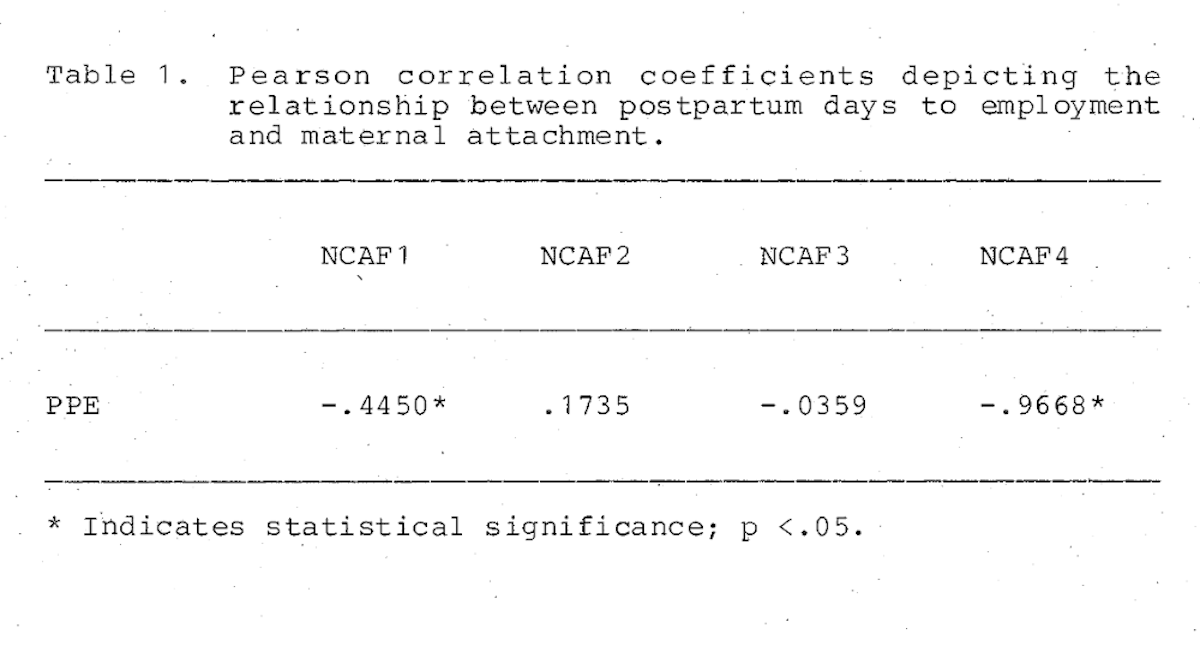
\includegraphics[scale=0.3]{workmomattach.png}

Let us assume known that all rapists have low childhood attachment security.  Then we can see that if we increase low attachment security in population, then the likelihood of rapists will increase.  We can then see that as wealth of the country increases, working mothers increase, the  attachment security decreases, rapists increase.

\section{Working Mothers predict Rape Rates}

\begin{verbatim}
> mod<-lm( log(Rape) ~ log(WorkMom), data=rp)
> summary(mod)

Call:
lm(formula = log(Rape) ~ log(WorkMom), data = rp)

Residuals:
     Min       1Q   Median       3Q      Max 
-2.01577 -0.78108 -0.01042  0.91365  1.66159 

Coefficients:
             Estimate Std. Error t value Pr(>|t|)  
(Intercept)   -3.1456     3.2232  -0.976   0.3436  
log(WorkMom)   1.5177     0.8376   1.812   0.0888 .
---
Signif. codes:  0 ‘***’ 0.001 ‘**’ 0.01 ‘*’ 0.05 ‘.’ 0.1 ‘ ’ 1

Residual standard error: 1.167 on 16 degrees of freedom
Multiple R-squared:  0.1703,	Adjusted R-squared:  0.1184 
F-statistic: 3.283 on 1 and 16 DF,  p-value: 0.08879
\end{verbatim}


\begin{thebibliography}{CCC}
\bibitem{K89}{Susan Thomas Kimes, {\em Working Mothers and Maternal Attachment: An Exploratory Study}, Ph.D. thesis U. Arizona 1989}
\end{thebibliography}
\end{document}
